\bexo
Tracer sur la même figure
\begin{itemize}
	\item $t\mapsto 2\sqrt{t}$
	\item $t\mapsto 1-\sqrt{3t}$
\end{itemize}

	\begin{center}
	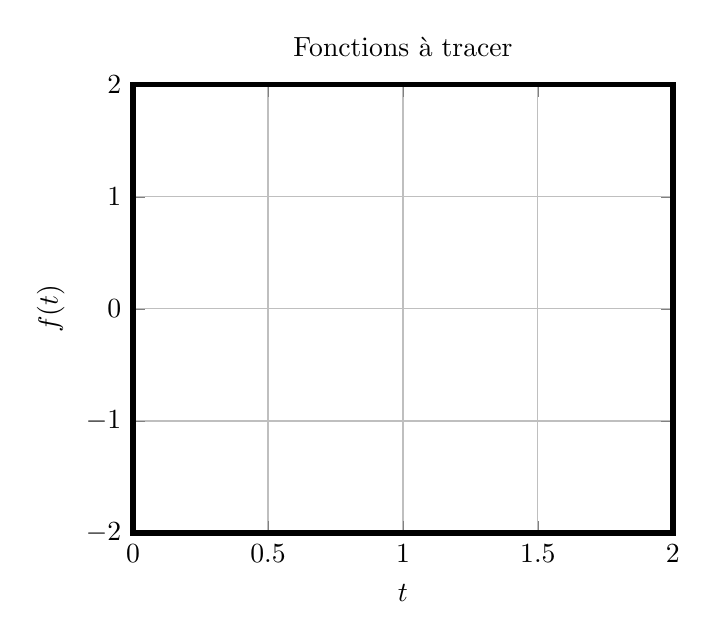
\begin{tikzpicture}
	  \begin{axis}[
				line width=2pt,
				legend columns=-1,
				title=Fonctions à tracer,
				xlabel={$t$},
				ylabel={$f(t)$},
				xmin=0,
				xmax=2,
				ymin=-2,
				ymax=2,
				legend to name=named,
				grid=major]
	  \end{axis}
	\end{tikzpicture}
\ref{named}
\end{center}




\eexo
\solution{
Les graphes des fonctions sont:\\

	\begin{center}
	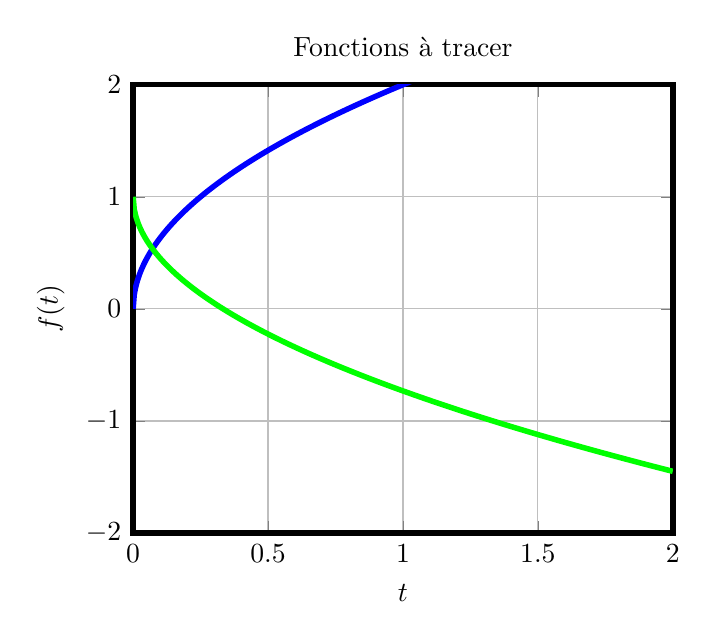
\begin{tikzpicture}
	  \begin{axis}[
				line width=2pt,
				legend columns=-1,
				title=Fonctions à tracer,
				xlabel={$t$},
				ylabel={$f(t)$},
				xmin=0,
				xmax=2,
				ymin=-2,
				ymax=2,
				legend entries={$2\sqrt{t}$,$1-\sqrt{3t}$},
				legend to name=named,
				grid=major]
		\addplot[blue] expression[domain=0:2,samples=500]{2*sqrt(x)};
		\addplot[green,samples=500] expression[domain=0:2]{1-sqrt(3*x)};
\end{axis}
	\end{tikzpicture}
		  \ref{named}
\end{center}


}
